
\begin{figure*}
{\footnotesize
\begin{center}
\begin{tabular}{|c|c|p{1.5in}|p{1.2in}|p{1.2in}|p{1.2in}|}\hline
Type &Acronym
 & Definition & Low-end
 &Medium &High-end\\\hline\hline
EM&acap  &  analyst capability  &  worst 15\% &   55\%  &  best 10\% \\\hline




EM&aexp   &   applications experience  &  2 months &   1 year  &  6 years\\\hline

SF&arch &  architecture or risk resolution  &  few interfaces
defined or few risk eliminated  &  most interfaces defined or most
risks eliminated   & all interfaces defined or all risks
eliminated\\\hline



EM&cplx   &   product complexity   & e.g. simple read/write
statements & e.g. use of simple interface widgets  &  e.g.
performance-critical embedded systems\\\hline


EM&data   &   database size \newline
(DB bytes/ Program SLOC) &
10 & 100 &    1000 \\\hline

EM&docu   &   documentation   & many life-cycle phases not
documented      & &  extensive reporting for each life-cycle phase\\\hline

SF&flex   &   development flexibility   & development process
rigorously defined & some guidelines, which can be relaxed & only
general goals defined\\\hline

EM&ltex   &  language and tool-set experience   & 2 months  &  1
year & 6 years \\\hline

EM&pcap   &   programmer capability  &  worst 15\%   & 55\%  &  best 10\% \\\hline



EM&pcon   &   personnel continuity \newline
(\% turnover per year) &
    48\% &    12\%  & 3\% \\\hline

EM&pexp   &  platform experience  &  2 months  &  1 year  &  6 years\\\hline


SF&pmat    &  process maturity  &  CMM level 1 &   CMM level 3  &  CMM level 5 \\\hline

SF&prec & precedentedness  &  we have never built this kind
of software before &    somewhat new &
thoroughly familiar \\\hline


EM&pvol   &   platform volatility  ($\frac{frequency~of~major~changes}{frequency~of~minor~changes}$) &
$\frac{12~months}{1~month}$   & $\frac{6~months}{2~weeks}$ &
$\frac{2~weeks}{2~days}$\\\hline



EM&rely   &   required
reliability &   errors mean slight inconvenience  &  errors are easily
recoverable   & errors can risk human life\\\hline




EM&ruse   &   required
reuse &   none   & across program  &  across  multiple product lines\\\hline

EM&sced  &    dictacted development\newline schedule &    deadlines moved closer to
75\% of the original estimate &  no change
&  deadlines moved back to  160\% of the original estimate\\\hline

EM&site   &   multi-site development   & some contact: phone, mail&
some email  &  interactive multi-media\\\hline

EM&stor  &    main storage constraints  \newline (\% of available
RAM) & N/A
 &   50\% &  95\% \\\hline

SF&team  &    team cohesion  &  very difficult interactions &
basically co-operative  &  seamless interactions\\\hline


EM&time  &    execution time constraints \newline (\% of available CPU) &
N/A&     50\%
   &  95\% \\\hline


EM&tool   &   use of software tools  &  edit,code,debug  &&      well
intergrated with lifecycle\\\hline

\end{tabular}
\end{center}
} \caption[Parameters of the COCOMO-II effort risk model]{Parameters of the COCOMO-II effort risk model; adapted
from~\protect\url{http://sunset.usc.edu/COCOMOII/expert_cocomo/drivers.html}.
``{\tt Stor}'' and ``{\tt time}'' score ``N/A"" for low-end values
since they have no low-end defined in COCOMO-II. ``SF'' denotes
``scale factors'' and ``EM'' denotes ``effort multipliers''.}
\label{fig:cparems}
\end{figure*}

The COCOMO project aims at developing an open-source,
public-domain software effort estimation model. The project has
collected information on 161 projects  from commercial, aerospace,
government, and non-profit organizations\cite{chulani99,boehm00b}. As of
1998, the projects represented in the database were of size 20 to
2000 KSLOC (thousands of lines of code) and took between 100 to
10000 person months to build.

COCOMO measures effort in calendar months where one month is 152
hours (and includes development and management hours). The core
intuition behind COCOMO-based estimation is that as systems grow
in size, the effort required to create them grows exponentially,
i.e. \mbox{$effort \varpropto KSLOC^x$}. More precisely:
\[
months=a*\left(KSLOC^{\left(0.91+\sum_{i=1}^{5}SF_i\right)}\right)*\left(\prod_{j=1}^{17}EM_j\right)
\]
where  $a$ is a domain-specific parameter, and KSLOC is  estimated
directly or computed from a function point analysis.
 $SF_i$ are the scale factors (e.g. factors
such as ``have we built this kind
 of system before?'') and
$EM_j$ are the cost drivers
(e.g.
required level of reliability). \fig{cparems} lists the scale drivers
and effort multipliers.

Software effort-estimation models like COCOMO-II should
 be tuned to
their  local domain. Off-the-shelf ``untuned'' models have been up
to 600\% inaccurate in their estimates, e.g. \cite[p165]{mukho92}
and~\cite{kemerer87}. However, tuned models can be far more
accurate.
 For example,~\cite{chulani99}
reports a study with a bayesian tuning algorithm using the COCOMO
project database. After bayesian tuning, a cross-validation study
showed that
 COCOMO-II model produced estimates that are within 30\% of the
 actuals,
 69\% of the time.

\begin{figure}
\begin{center}
\begin{tabular}{c|c|c}
$\times$ & $\surd$ & $\surd\surd$ \\\hline
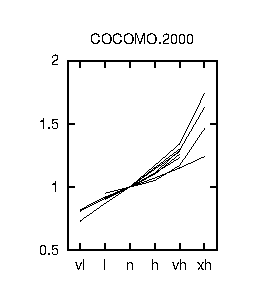
\includegraphics[width=2.5cm]{coc2000down.eps}&
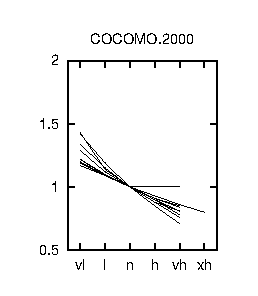
\includegraphics[width=2.5cm]{coc2000up.eps}&
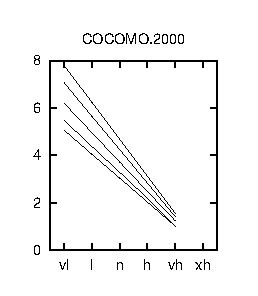
\includegraphics[width=2.5cm]{coc2000cliff.eps}\\

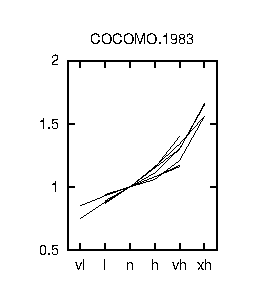
\includegraphics[width=2.5cm]{coc1983down.eps}&
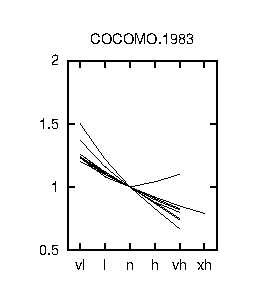
\includegraphics[width=2.5cm]{coc1983up.eps}&
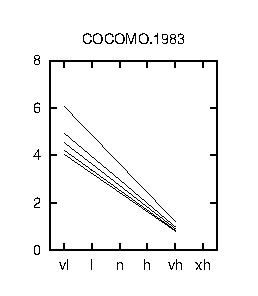
\includegraphics[width=2.5cm]{coc1983cliff.eps}\\

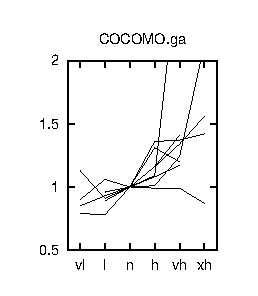
\includegraphics[width=2.5cm]{cocgadown.eps}&
\includegraphics[width=2.5cm]{cocgaup.eps}&
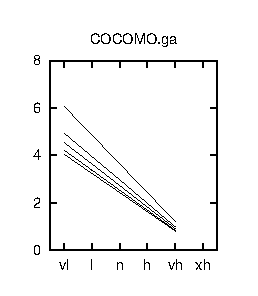
\includegraphics[width=2.5cm]{cocgacliff.eps}
\end{tabular}
\end{center}
\caption{Influence of different COCOMO parameters}
\end{figure}


\begin{center}
{\scriptsize
\begin{tabular}{ccc|ccc|ccc}
&$\times$&&&$\surd$&&&$\surd\surd$ &\\\hline
2000&ga&1983&2000&ga&1983&2000&ga&1983\\\hline
-&tool&-&tool&-&tool&team&team&team\\
time&time&time&site&site&site&prec&prec&prec\\
stor&stor&stor&sced&sced&sced&pmat&pmat&pmat\\
ruse&ruse&ruse&-&pvol&-&flex&flex&flex\\
rely&rely&rely&pexp&pexp&pexp&arch&arch&arch\\
pvol&-&pvol&pcon&pcon&pcon&&&\\
docu&docu&docu&pcap&pcap&pcap&&&\\
data&data&data&ltex&ltex&ltex&&&\\
cplx&cplx&cplx&aexp&aexp&aexp&&&\\
&&&acap&acap&acap&&&
\end{tabular}}
\end{center}
